\documentclass{examen}

\begin{document}
\modulo{Lenguajes de marcas. Tema 6 XQuery}

Dado el archivo XML que se puede encontrar al final, extraer la informaci�n pedida en los siguientes enunciados usando el lenguaje que se indique

\pregunta{Mostrar la media global de la cantidad de partes suministradas p1, p2 y p4 (Debe salir un solo resultado)}{2}



\pregunta{Averiguar la media de partes que reciben los proyectos Clasificador y OCR. Deben salir dos resultados}{1.5}
\pregunta{Mostrar los nombres de proyecto, los codigos de parte que reciben y la cantidad de dichas partes que reciben}{1.5}
\pregunta{Devolver el recuento de proveedores que han suministrado alguna de estas partes: p1, p2, p3 o p6. Solo debe salir un resultado}{1}


\pregunta{Indicar los nombres de proveedores y los nombres de proyecto a los que suministran piezas. No importa si hay repetidos}{1}
\pregunta{Indicar cuantos proveedores hay cuyo estado sea 20 y su ciudad sea Londres.  Solo debe salir un resultado}{1}
\pregunta{Mostrar los nombres de los proveedores junto a la media de partes rojas que suministran}{2}


\break 
\begin{verbatim}
<datos>
    <proveedores>
        <proveedor numprov="v1">
            <nombreprov>Smith</nombreprov>
            <estado>20</estado>
            <ciudad>Londres</ciudad>
        </proveedor>
        ... omitido ...
    </proveedores>
    <partes>
        <parte numparte="p1">
            <nombreparte>Tuerca</nombreparte>
            <color>Rojo</color>
            <peso>12</peso>
            <ciudad>Londres</ciudad>
        </parte>
        ... omitido ...
    </partes>
    <proyectos>
        <proyecto numproyecto="y1">
            <nombreproyecto>Clasificador</nombreproyecto>
            <ciudad>Paris</ciudad>
        </proyecto>
        ... omitido ...
    </proyectos>
    <suministros>
        <suministra>
            <numprov>v1</numprov>
            <numparte>p1</numparte>
            <numproyecto>y1</numproyecto>
            <cantidad>200</cantidad>
        </suministra>
        <suministra>
            <numprov>v1</numprov>
            <numparte>p1</numparte>
            <numproyecto>y4</numproyecto>
            <cantidad>700</cantidad>
        </suministra>
        ... omitido ...
    </suministros>
</datos>
\end{verbatim}

\begin{figure}[h]
    \caption{Esquema de la base de datos}
    \label{figura1}
    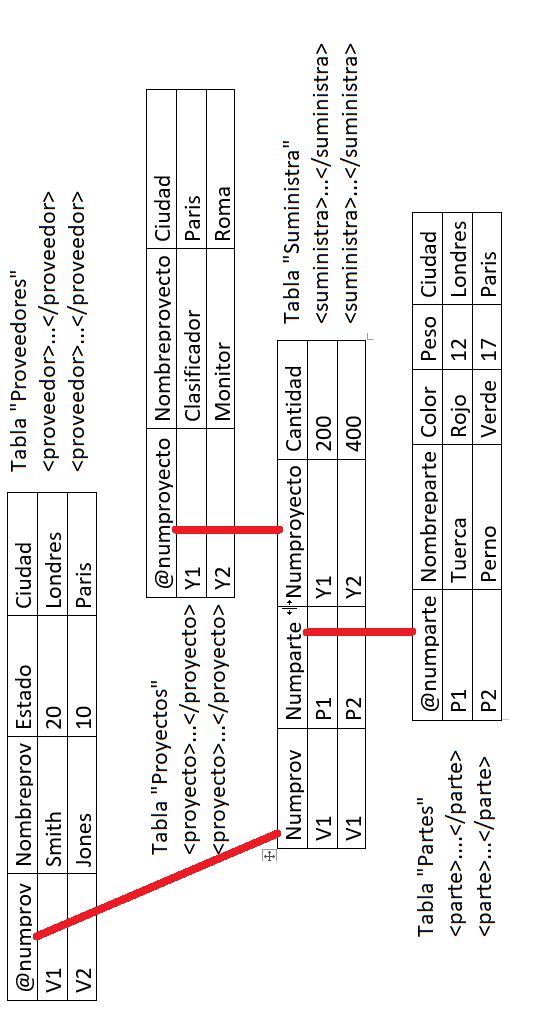
\includegraphics[width=\linewidth]{examen-img/BaseDatosProveedoresPartesProyectos.png}
\end{figure}

\end{document}
